
\vspace{-0.06in}
\section{Experiments}
\vspace{0.04in}
\subsection{Experimental Setup}



\paragraph{Datasets and Evaluation Metrics.}

To ensure comprehensive evaluation across diverse scenarios, we conduct experiments on nine datasets from multiple domains with distinct temporal characteristics (Table~\ref{tab:data_statistics}). These include ETT \citep{zhou2021informer} for 2016--2018 electricity load records, Exchange \citep{lai2018modeling} for 1990--2016 foreign exchange rates, Wind \citep{lai2018modeling} for 2020--2021 wind measurements, AQ \citep{zhang2017cautionary} for four-year air quality records, and NASDAQ \citep{feng2019temporal} for stock market series including prices and trading volumes.
We report MSE between predictions and ground truth under a 96-step forecasting horizon for all datasets, except NASDAQ, which uses a 36-step horizon.

% To ensure comprehensive evaluation across diverse scenarios, we conduct experiments in nine datasets spanning multiple domains with distinct temporal characteristics and data attributes (detailed in Table  \ref{tab:data_statistics}). These include: the ETT dataset \citep{zhou2021informer} capturing 2016-2018 electricity load records, Exchange \citep{lai2018modeling} tracking 1990-2016 foreign exchange rates, Wind \citep{lai2018modeling} with 2020-2021 wind measurements captured, AQ \citep{zhang2017cautionary} providing four-year air quality data, NASDAQ \citep{feng2019temporal} provides complete stock market series including opening/closing prices, trading volumes, and daily high-low values.
% All datasets were evaluated using Mean Squared Error (MSE) under a 96-step prediction setting, except NASDAQ which uses a 36-step configuration, with results reported as the MSE between predictions and ground truth.



\paragraph{Baselines.}

Our representative baselines include various competitive methods:
Autoformer \citep{wu2021autoformer}, PatchTST \citep{nie2022time}, DLinear \citep{zeng2023transformers}, iTransformer \citep{liu2023itransformer}, TimeXer \citep{wang2024timexer}, TimeMixer \citep{wang2024timemixer}, 
WPMixer \citep{murad2025wpmixer}, Moment \citep{goswami2024moment}, TimesFM-2.5 \citep{das2024decoder} and Chronos-2 \citep{ansari2025chronos}. For recent LLM-based approaches, we include CrossTimeNet \citep{crossTimeNet}, GPT4TS \citep{zhou2023one}, TimeLLM \citep{jin2023time}, and DeepSeek-R1 \citep{deepseekR1} for zero-shot inference.



\paragraph{Implementation Details.}
% For baseline methods, we use Adam \citep{kingma2014adam} as the default optimizer across all the experiments.
% All the experiments are implemented by PyTorch \citep{paszke2019pytorch} and are conducted for three runs with a fixed random seed on a single NVIDIA RTX 4090D 24GB GPU.
% Unlike traditional TSF methods that often require normalization, we conduct experiments in the original numerical space.
% Unlike traditional TSF methods, we conduct experiments in the original numerical space to preserve physical magnitudes essential for LLM reasoning and zero-shot generalization.
% For Time-R1, we keep the time-series values in their original numerical scale as model inputs and outputs, so that the LLM can access physically meaningful magnitudes during reasoning. For baseline forecasting models, we follow their standard or recommended preprocessing protocols, including normalization when applicable, and report all metrics after mapping predictions back to the original scale.
% Please refer to Appendix F for the results regarding the normalized evaluation. 
% For \Ours, we use Qwen2.5-7B-Instruct as the backbone. In SFT, we train on 3000 synthetic samples with a learning rate of 5e-5 for one epoch. In RL, we implement GRIP using the Verl framework \citep{verl} with vLLM for generation, $\epsilon=0.2$ and $\beta=0.04$; group size $G=16$, $k=3$. The batch size is 16, learning rate is 1e-6, policy temperature is 1, and max completion length is 8000. Both stages are run on a 4-GPU A800 cluster. For DeepSeek-R1, we apply its prompt directly to time series prediction without training. 
% Time-R1 is trained only on ETTh1 and generalized to other datasets without fine-tuning, whereas baseline methods require separate models per dataset.


% For Time-R1, we keep the time-series values in their original numerical scale as model inputs and outputs, so that the LLM can access physically meaningful magnitudes during reasoning. For baseline forecasting models, we follow their standard or recommended preprocessing protocols, including normalization when applicable, and report all metrics after mapping predictions back to the original scale.

Tables~\ref{tab:main_results_mse} and~\ref{tab:main_results_mae} report MSE and MAE on each dataset's original scale, with all results averaged over three runs using different random seeds. Baselines follow their official or commonly adopted experimental configurations, with predictions inverse-transformed before evaluation when normalization is used. For \Ours, we keep the model-facing time-series values in the original numerical scale as both inputs and outputs, allowing the LLM to access physically meaningful magnitudes during reasoning.

For \Ours, we use Qwen2.5-7B-Instruct as the backbone. In SFT, we train on 3000 synthetic samples with a learning rate of 5e-5 for one epoch. In RL, we implement GRIP using the VeRL framework \citep{verl} with vLLM for generation, $\epsilon=0.2$ and $\beta=0.04$; group size $G=16$, $k=3$. The batch size is 16, learning rate is 1e-6, policy temperature is 1, and max completion length is 8000. Both stages are run on a 4-GPU A800 cluster. For DeepSeek-R1, we apply its prompt directly to time series prediction without training. 


% \begin{table}[th]
%     \centering
%     \large
%     \caption{Statistics information of experimental datasets.}
%     % \vspace{-0.06in}
%     \renewcommand{\arraystretch}{1.3}
%     \scalebox{0.7}{
%     \begin{tabular}{cccccccccc}
%     \hline
%         Dataset & Domain & Timestamps & Features &  Frequency \\ 
%         \hline
%         ETTh1\&ETTh2 & Electricity & 17,420 & 7 &  1 hour \\ 
%         ETTm1\&ETTm2 & Electricity & 69,680 & 7 &   15 mins \\
%         AQWan\&AQShunyi & Environment & 35,064 & 11 & 1 hour  \\ 
%         Exchange & Economy & 7,588 & 8 &  1 day  \\ 
%         Wind & Energy & 48,673 & 7 &   15 mins \\ 
%         NASDAQ & Stock & 1,244 & 5 &  1 day \\ 
%     \hline
%     \end{tabular}
%     }
%     \label{tab:data_statistics}
% \end{table}



\begin{table}[t]\centering
    \caption{Statistics information of experimental datasets.}
    \renewcommand{\arraystretch}{1.2}
    \vspace{-0.1in}
    \label{tab:data_statistics}
    \resizebox{0.48\textwidth}{!}{
    \large
    \begin{tabular}{cccccccccc}
        \toprule
        Dataset & Domain & Timestamps & Features &  Frequency \\ 
        \hline
        ETTh1\&ETTh2 & Electricity & 17,420 & 7 &  1 hour \\ 
        ETTm1\&ETTm2 & Electricity & 69,680 & 7 &   15 mins \\
        AQWan\&AQShunyi & Environment & 35,064 & 11 & 1 hour  \\ 
        Exchange & Economy & 7,588 & 8 &  1 day  \\ 
        Wind & Energy & 48,673 & 7 &   15 mins \\ 
        NASDAQ & Stock & 1,244 & 5 &  1 day \\ 
        \bottomrule
    \end{tabular}
    }
    \vspace{-0.2in}
\end{table}


\begin{figure*}[htp]
    \centering
    \begin{subfigure}[b]{0.23\textwidth}
        \centering
        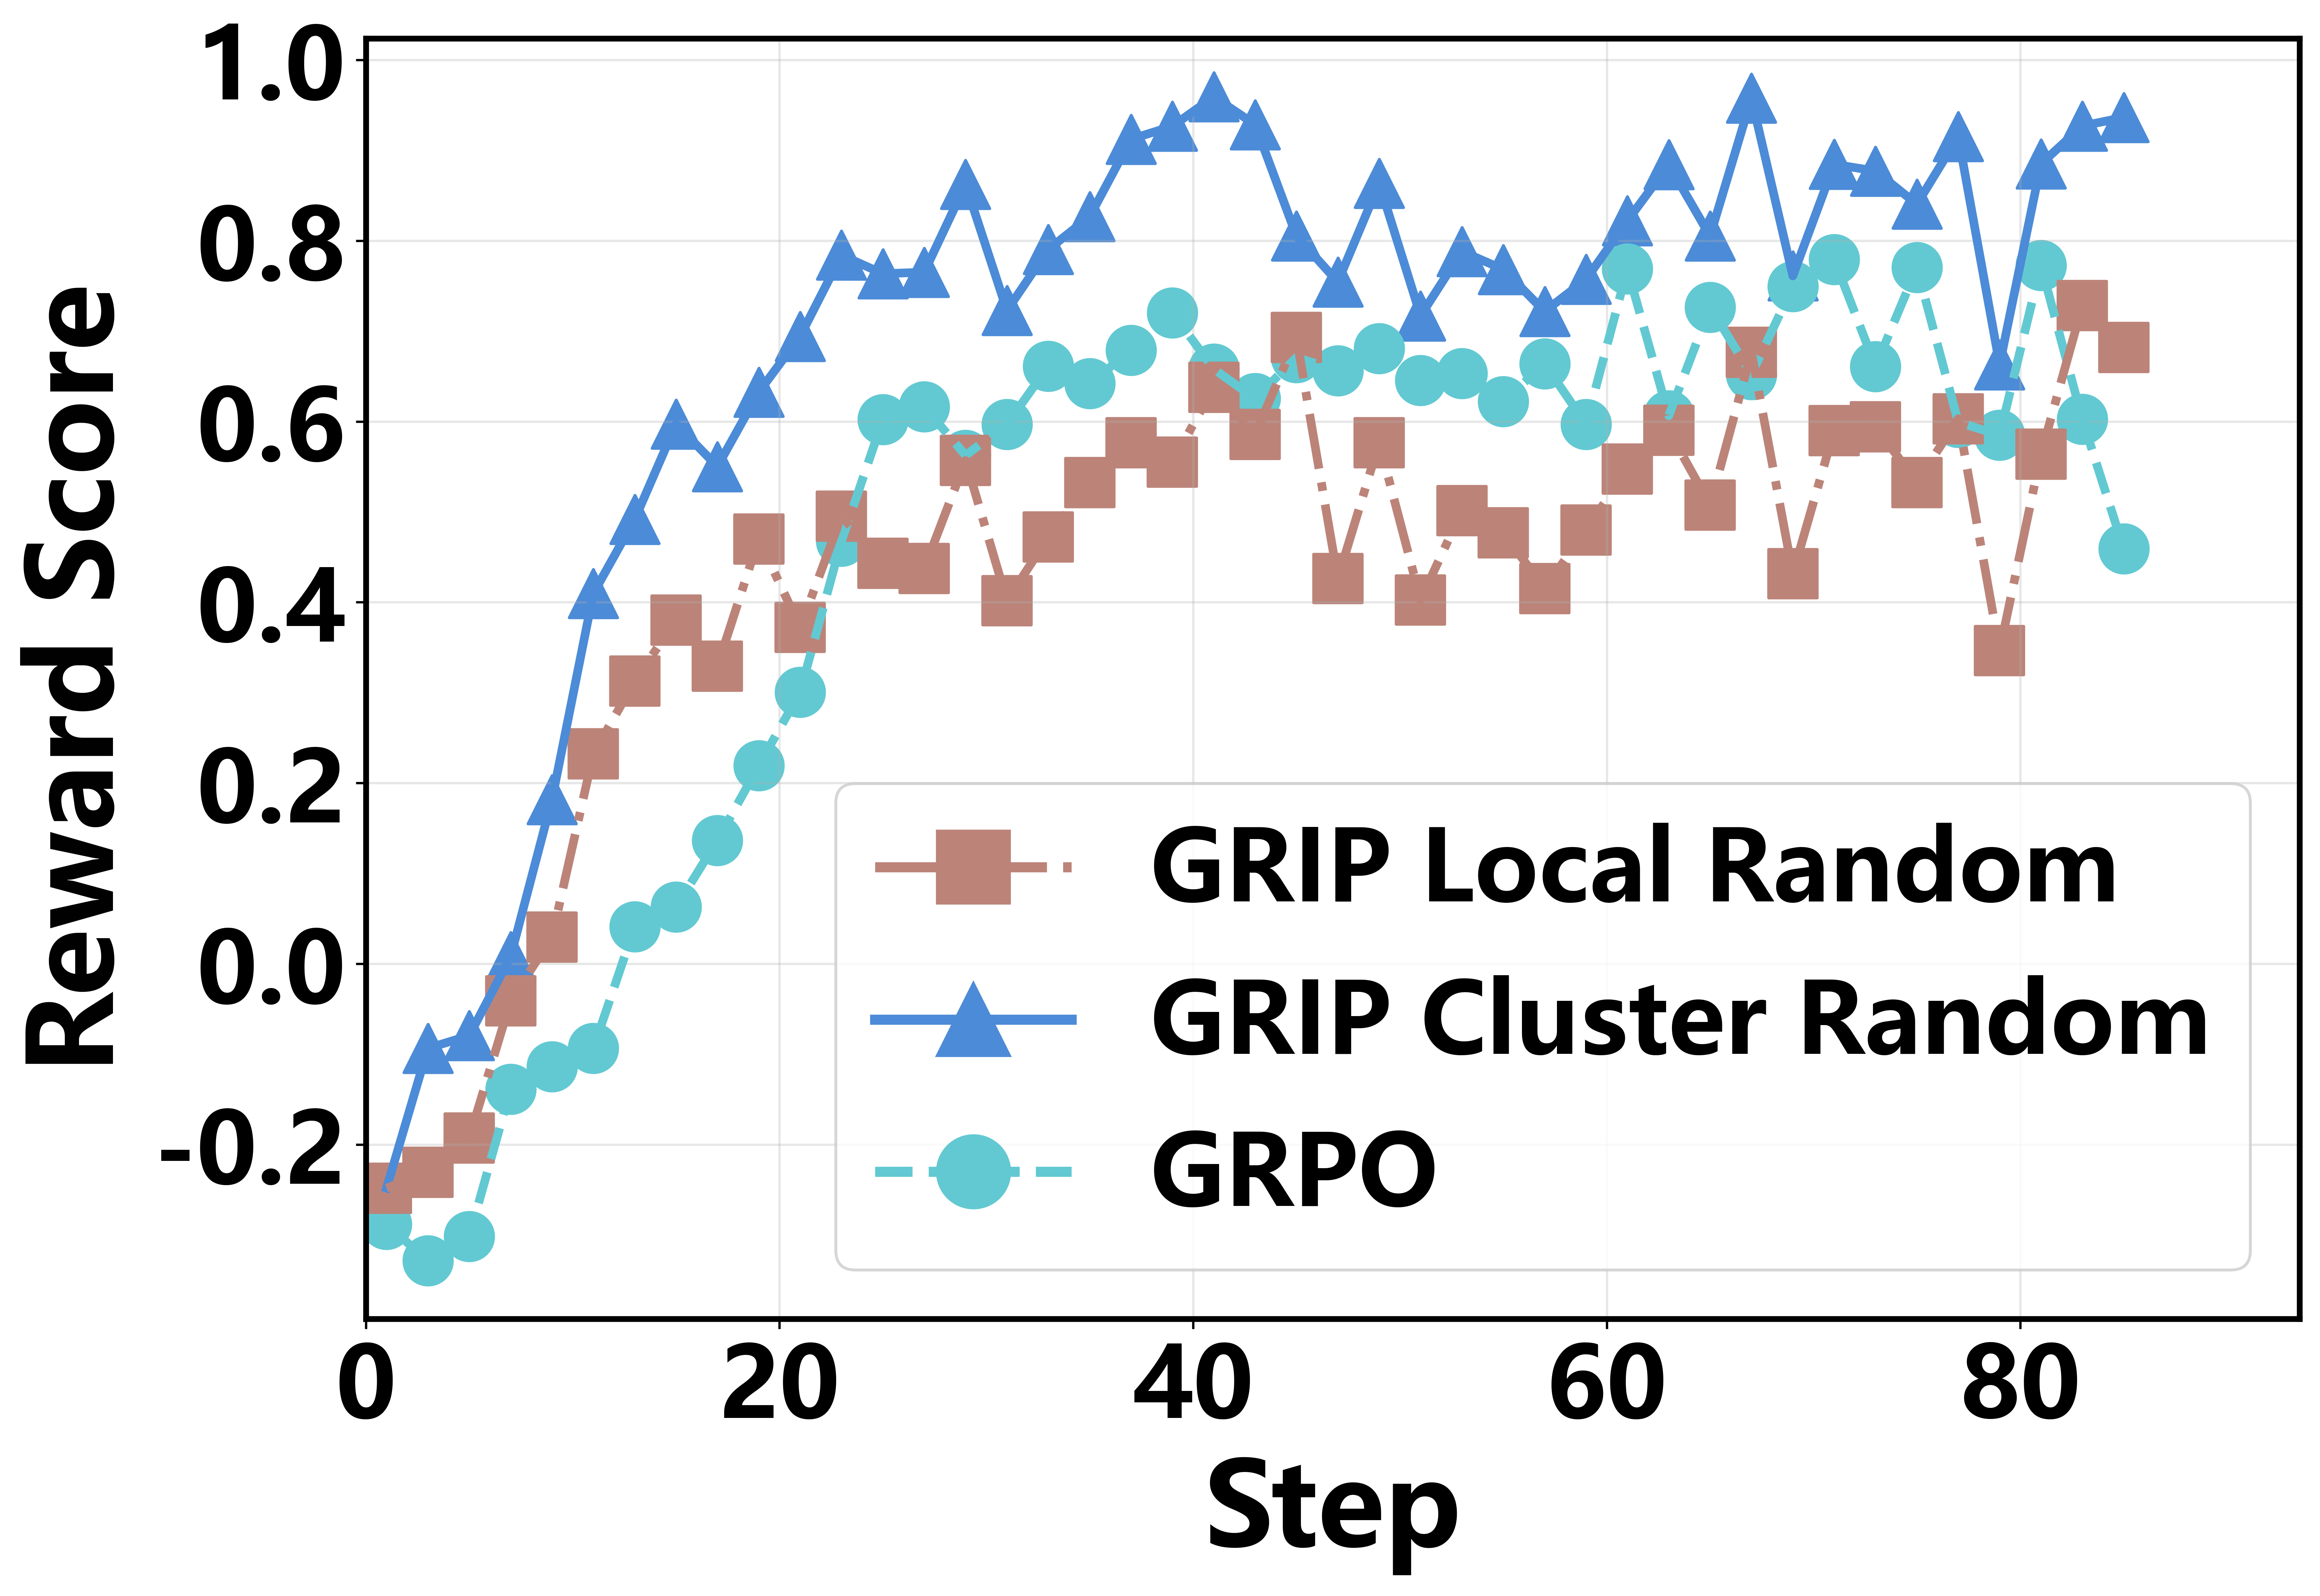
\includegraphics[width=\textwidth]{images/compare/GRIP_work.png}
        % \vspace{-0.1in}
        \caption{GRIP vs. GRPO}
        \label{fig:compare_a}
    \end{subfigure}
    \hfill
    \begin{subfigure}[b]{0.23\textwidth}
        \centering
        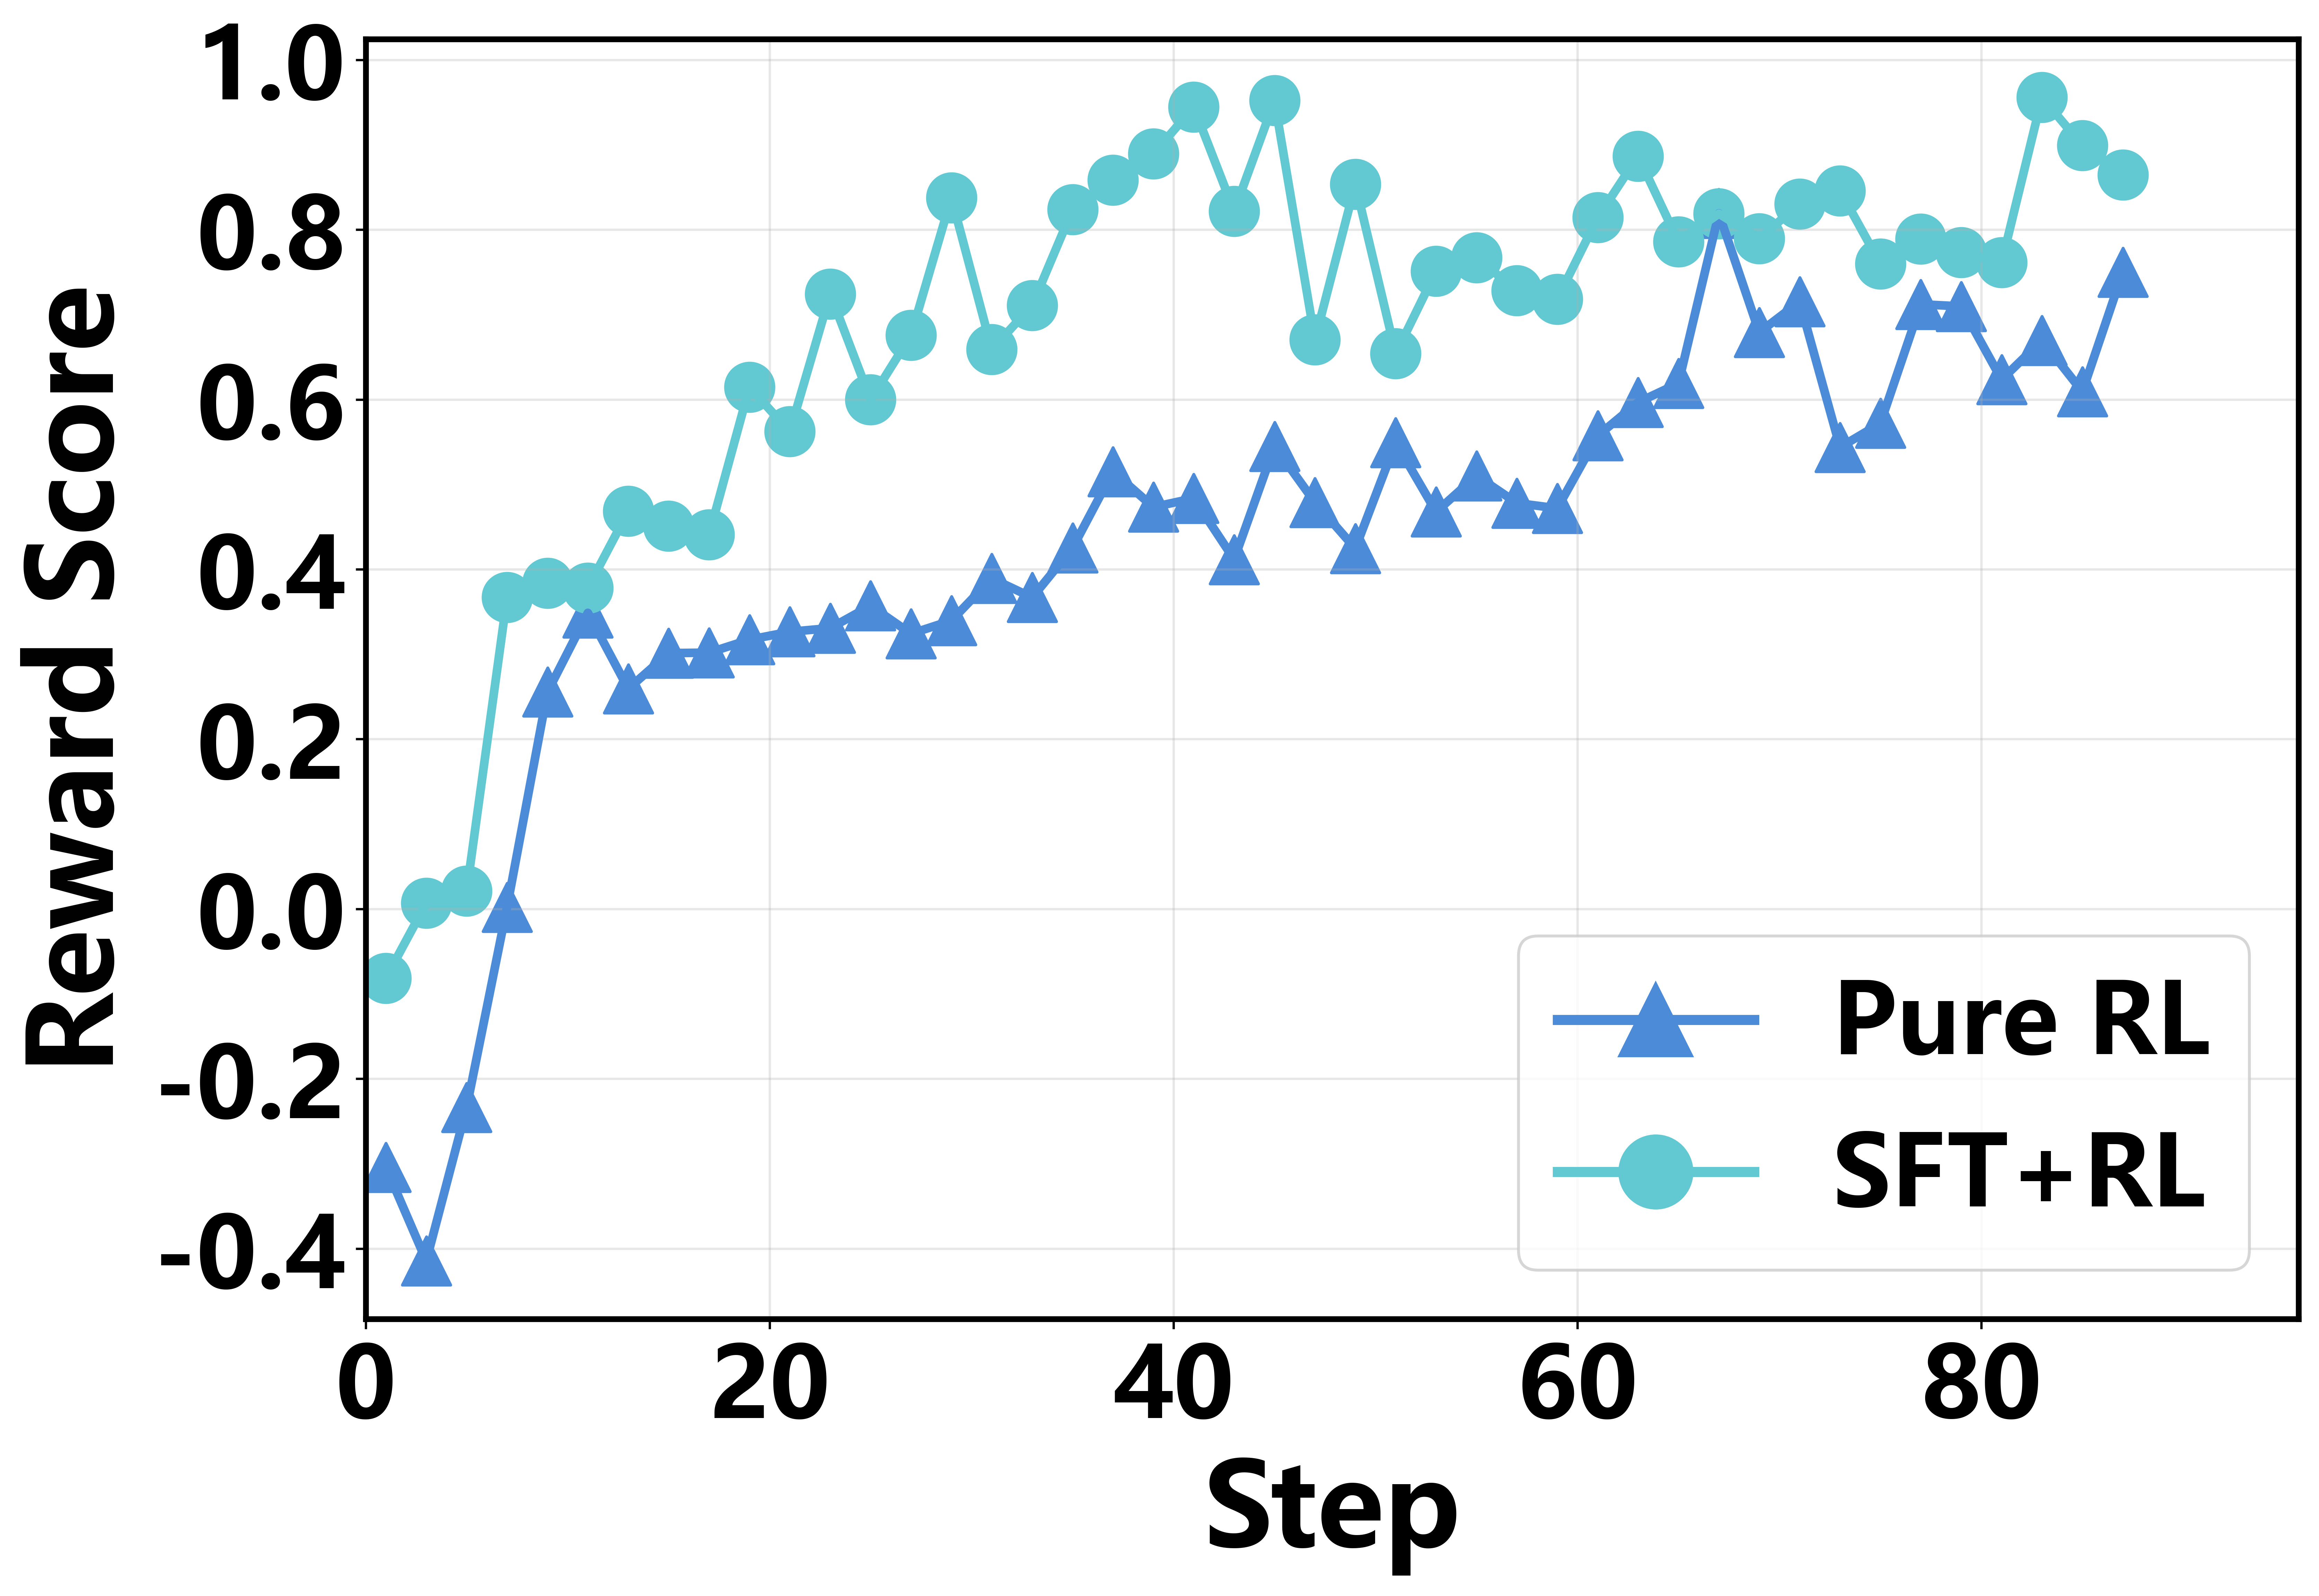
\includegraphics[width=\textwidth]{images/compare/SFT_RL.png}
        % \vspace{-0.1in}
        \caption{RL vs. SFT + RL}
        \label{fig:compare_b}
    \end{subfigure}
    \hfill
    \begin{subfigure}[b]{0.23\textwidth}
        \centering
        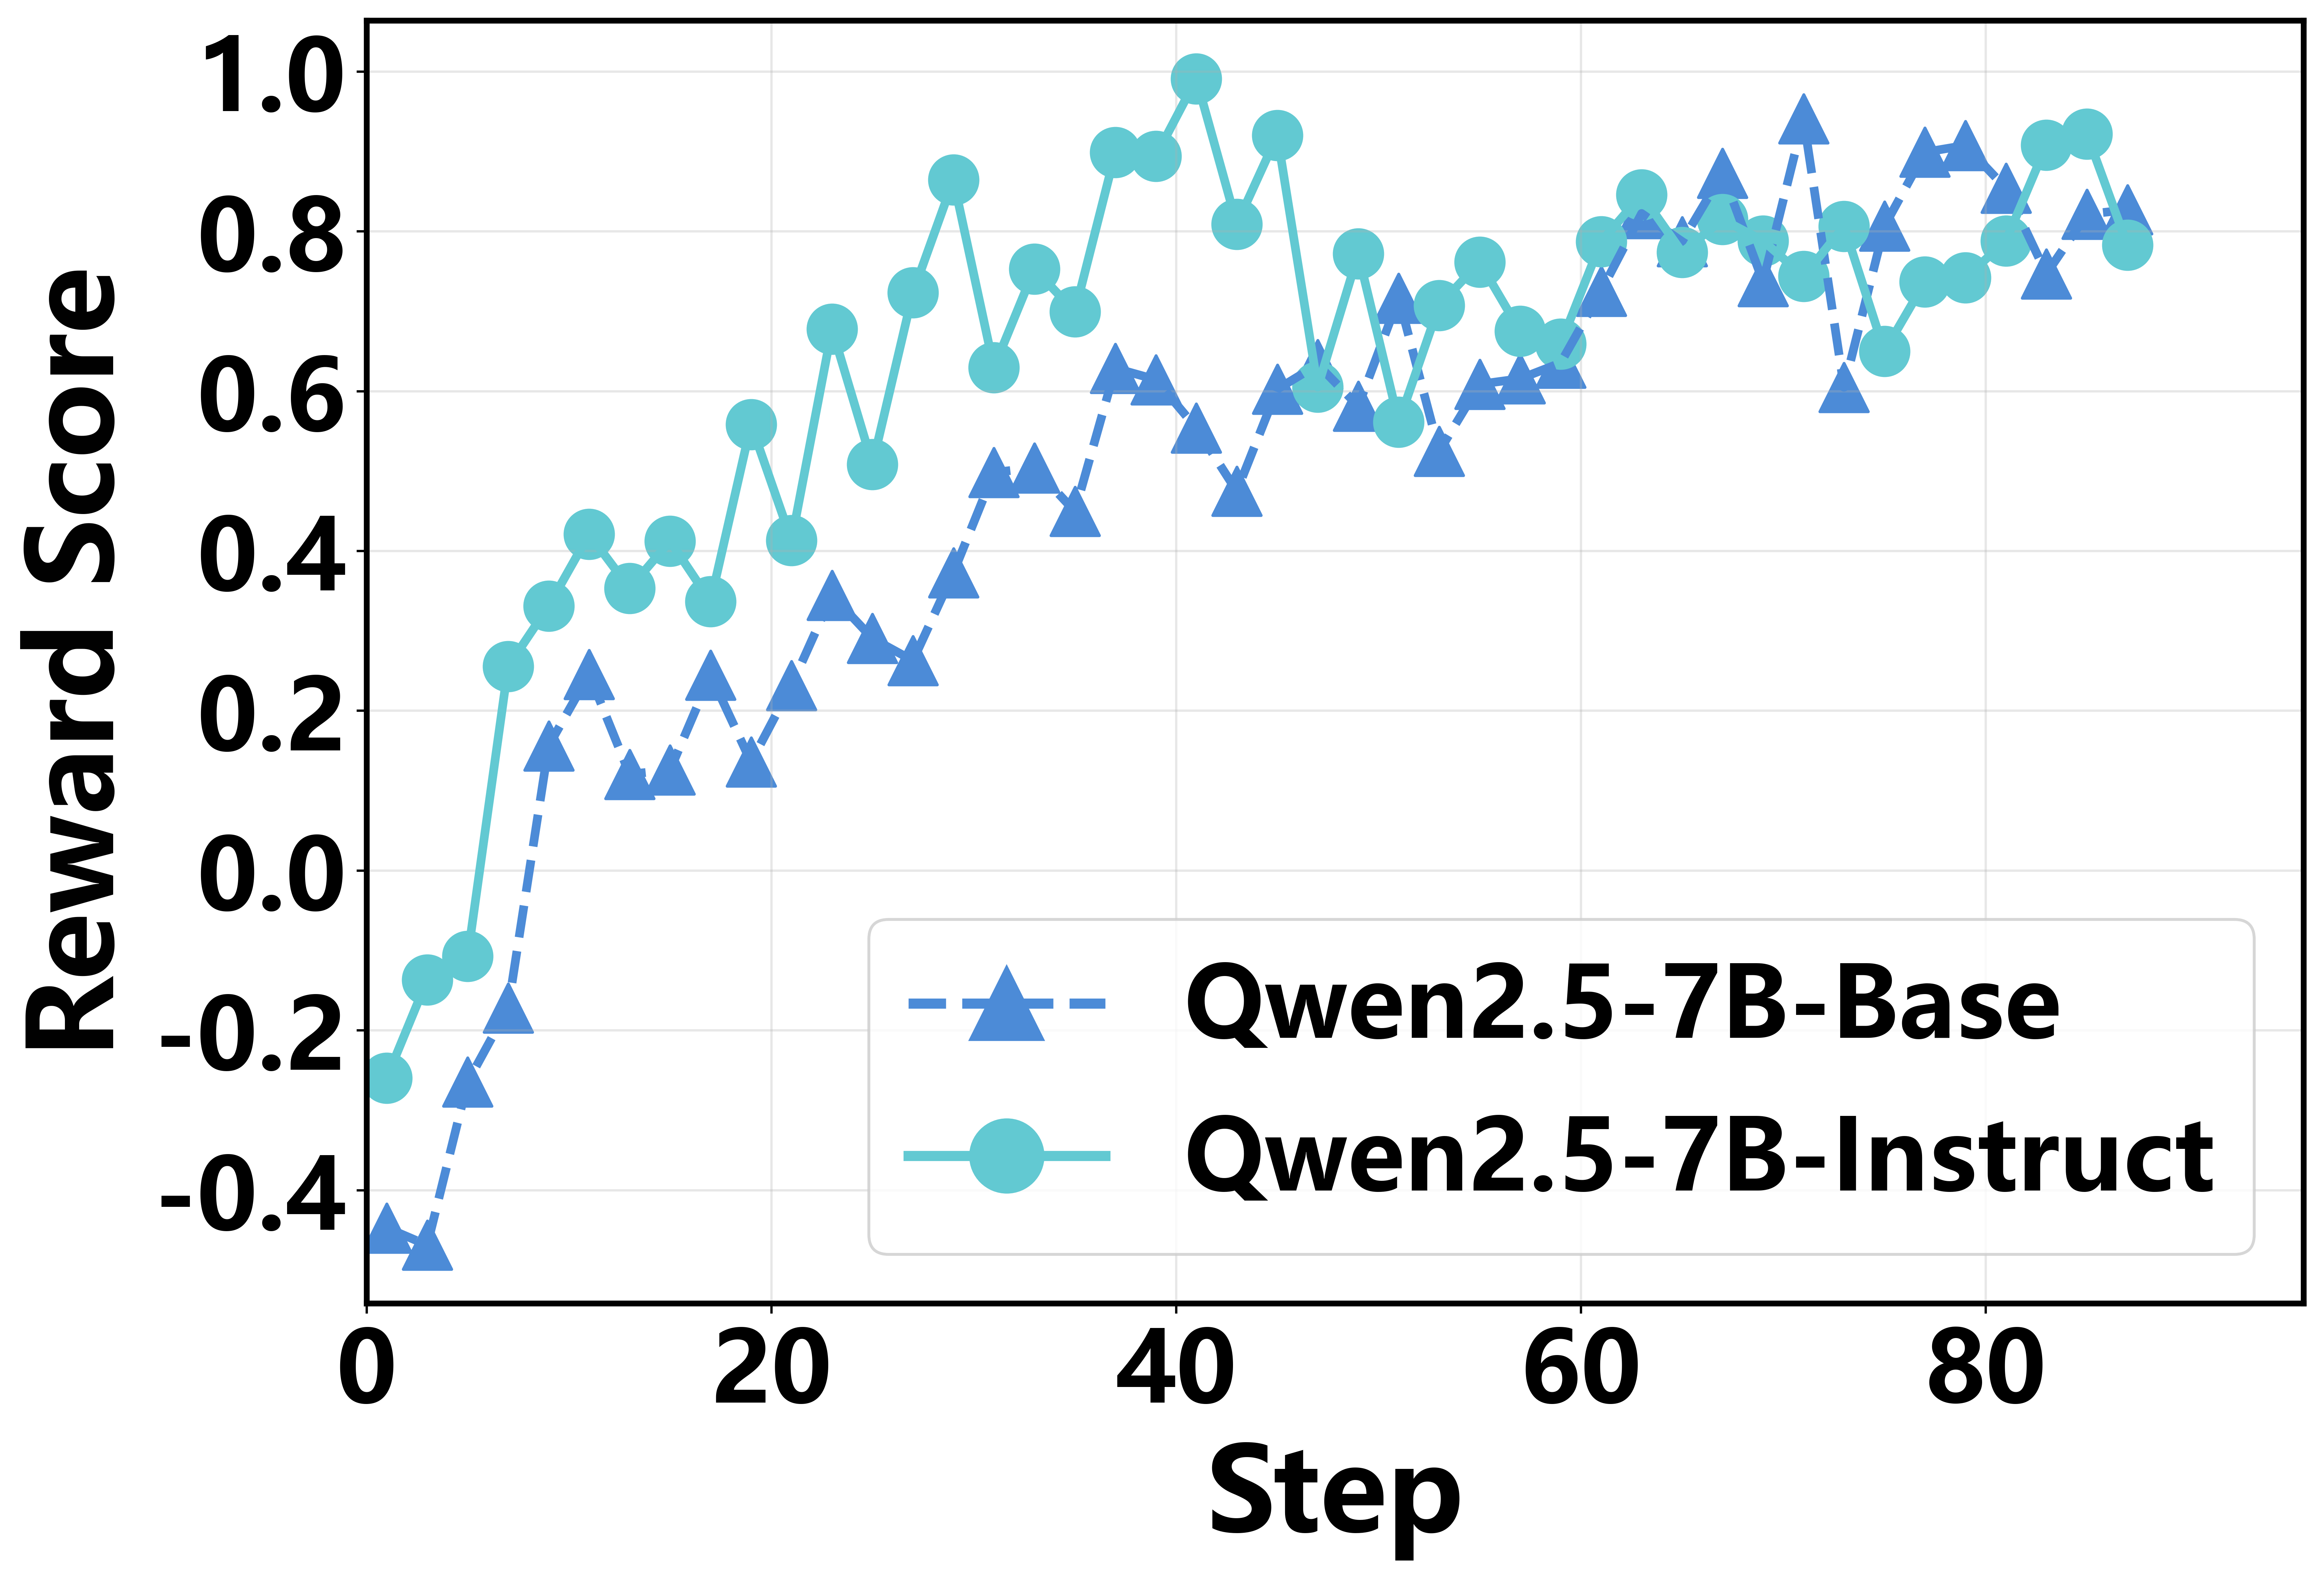
\includegraphics[width=\textwidth]{images/compare/Base_Instruct.png}
        % \vspace{-0.1in}
        \caption{Base vs. Instruct}
        \label{fig:compare_c}
    \end{subfigure}
    \hfill
    \begin{subfigure}[b]{0.23\textwidth}
        \centering
        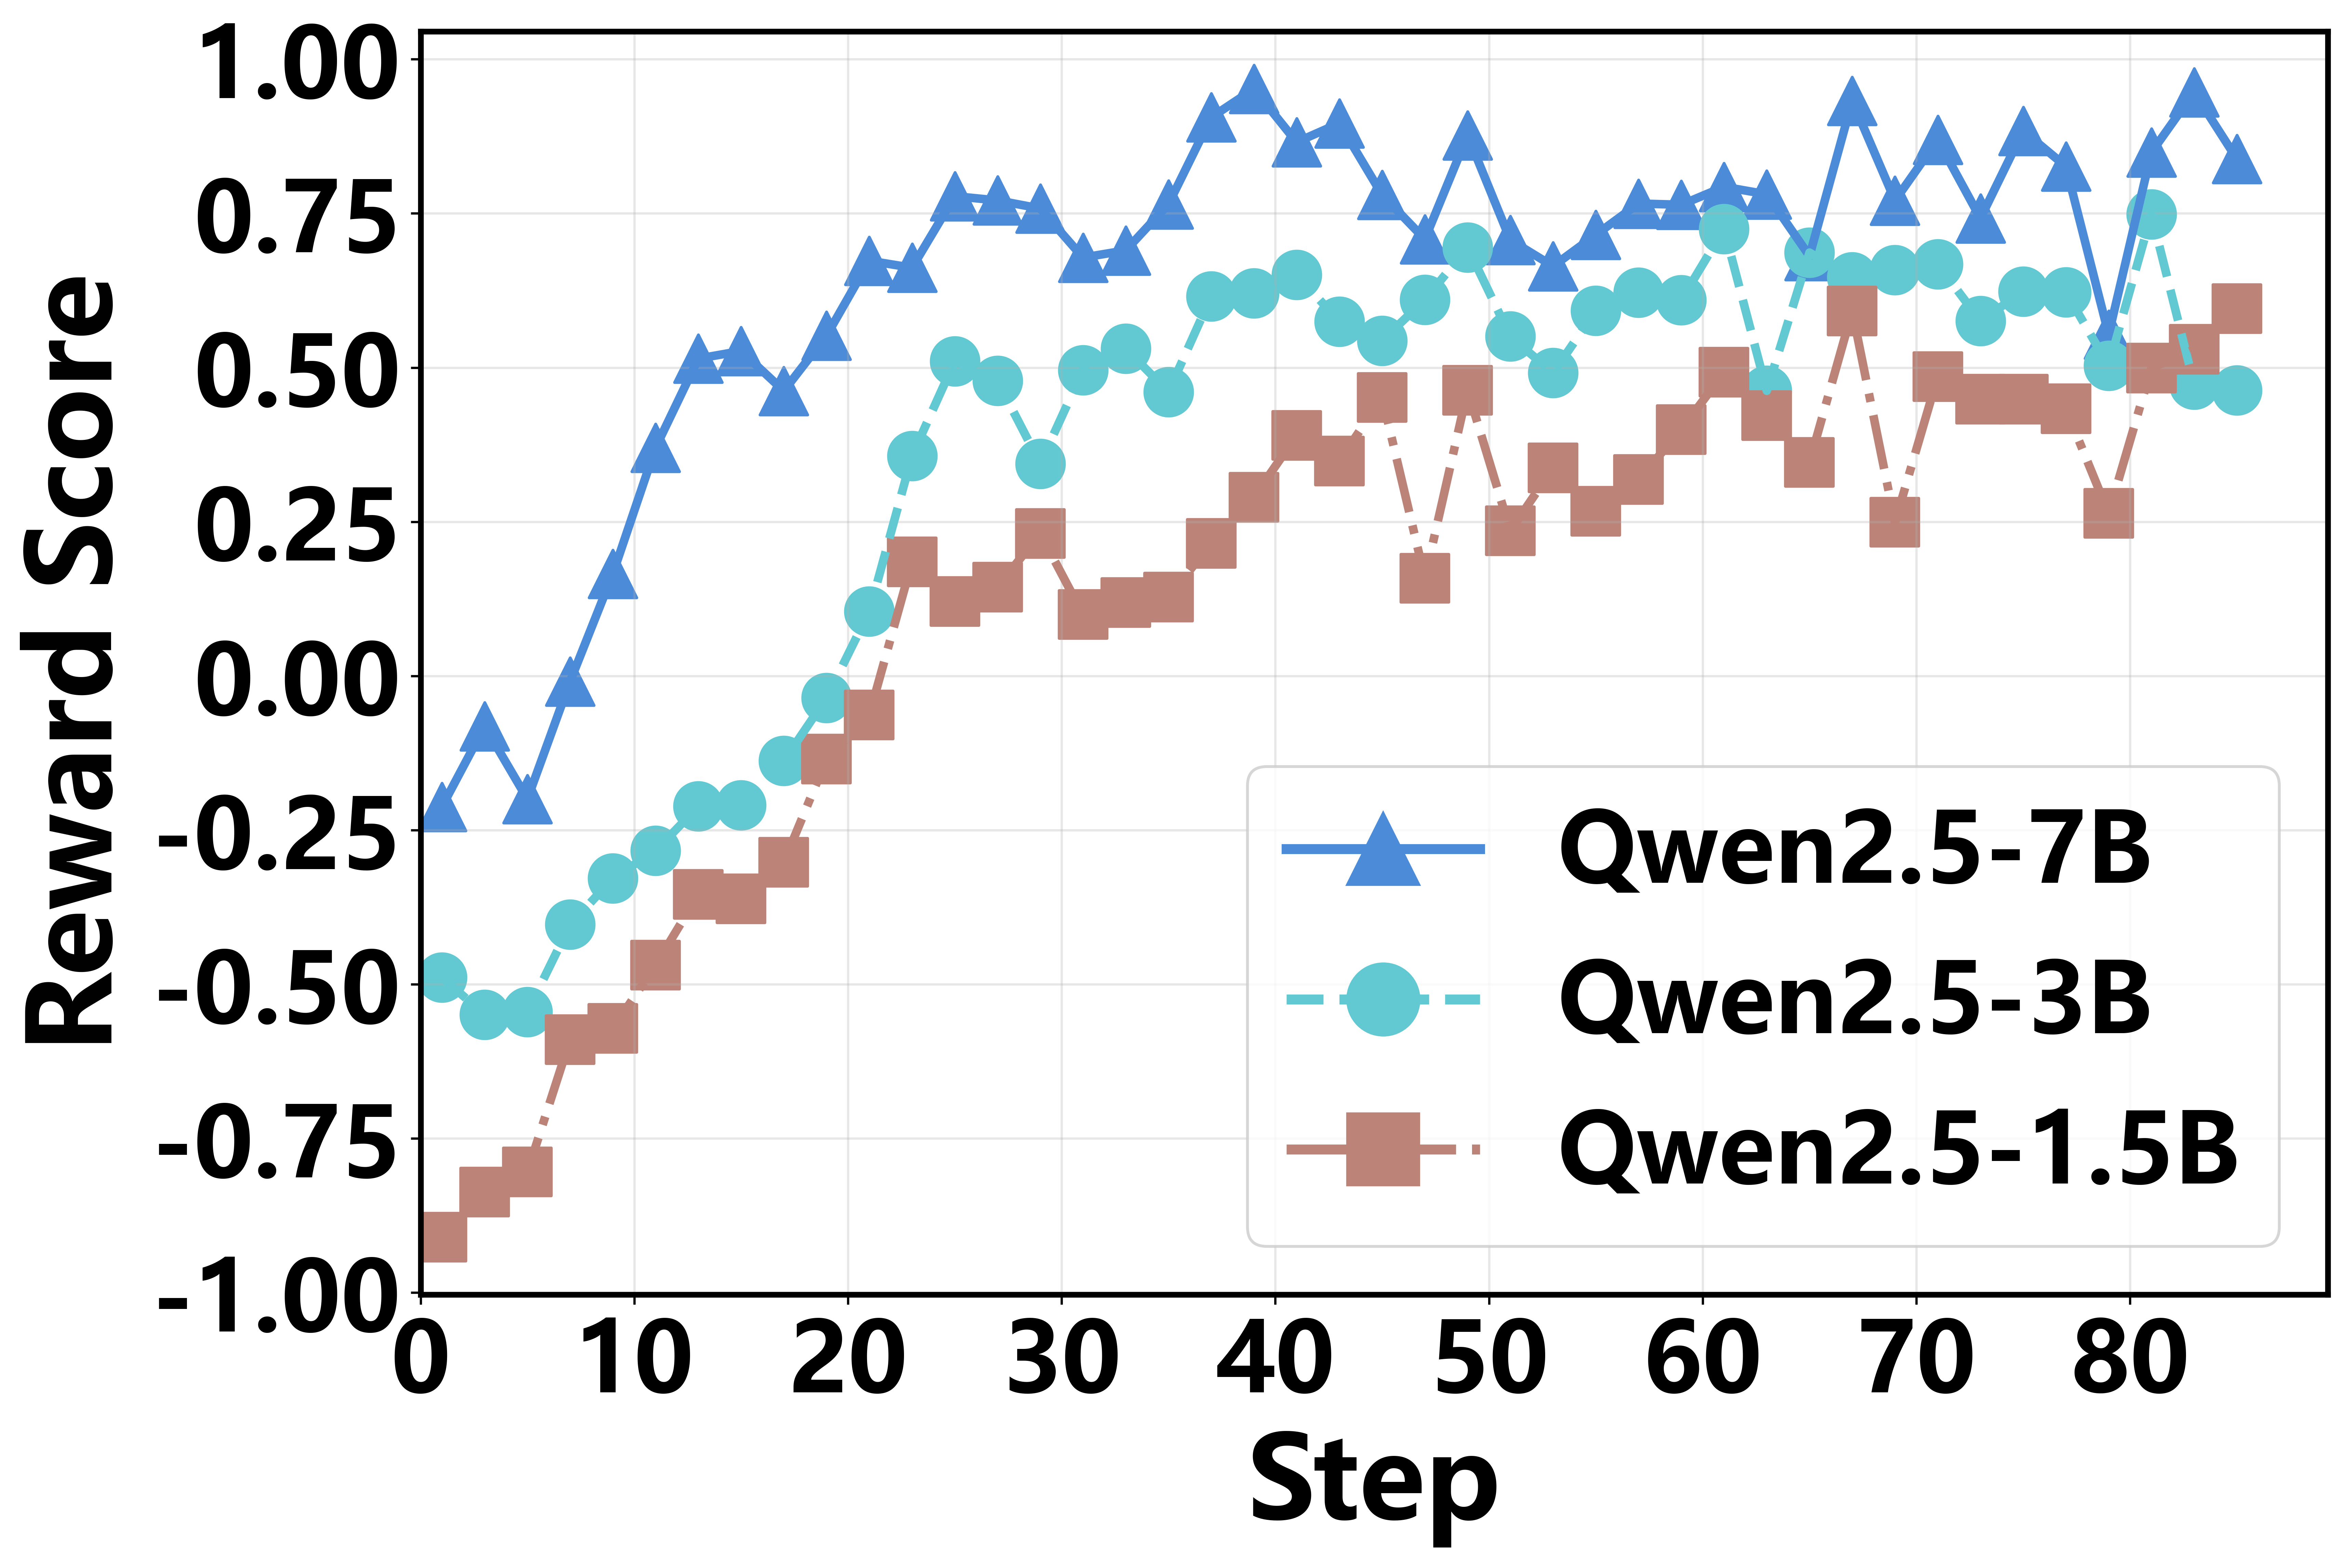
\includegraphics[width=\textwidth]{images/compare/model_scale.png}
        % \vspace{-0.1in}
        \caption{Model Scaling}
        \label{fig:compare_d}
    \end{subfigure}

    \caption{(a) GRIP vs. GRPO: GRIP converges faster with slightly higher final performance. (b) RL vs. SFT+RL: SFT+RL achieves faster initial convergence and superior final performance. (c) Base vs. Instruct: Instruct model enables faster early reward growth, though base model achieves higher final reward. (d) Model Scaling: Larger models achieve higher final rewards, indicating stronger time-series reasoning and forecasting capability.}
    \label{fig:compare}

\end{figure*}
\begin{table*}[t]\centering
\centering

\caption{Ablation study on Training Strategies, Reward Design, and Template Components.} 

\renewcommand{\arraystretch}{1.05}
\resizebox{0.85\textwidth}{!}{
\begin{tabular}{llcccccc}
\toprule
 & \multicolumn{1}{l}{\multirow{2}{*}{Method}} & \multicolumn{2}{c}{ETTh1} & \multicolumn{2}{c}{ETTm2} & \multicolumn{2}{c}{Wind} \\
\cmidrule(r{2pt}){3-4}
\cmidrule(l{2pt}r{2pt}){5-6}
\cmidrule(l{2pt}){7-8}
 & \multicolumn{1}{c}{}                  & MSE          & MAE        & MSE         & MAE         & MSE         & MAE        \\
\midrule

\cellcolor{lightgray!30}Full Model & \cellcolor{lightgray!30}\Ours                               & \cellcolor{lightgray!30}\textbf{5.8752}       & \cellcolor{lightgray!30}\textbf{1.2325}     & \cellcolor{lightgray!30}\textbf{5.6673}       & \cellcolor{lightgray!30}\textbf{1.3771}     & \cellcolor{lightgray!30}\textbf{1353.9381}    & \cellcolor{lightgray!30}\textbf{15.1095}   \\
\midrule
\multirow{2}{*}{\begin{tabular}[l]{@{}l@{}}Training\\ Strategies\end{tabular}} &\textit{w/o} SFT     & 6.3558       & 1.4278     & 6.3673       & 1.4850     & 1632.6491    & 16.7903   \\
 &\textit{w/o} RL                                & 13.2196      & 1.7820     & 12.5940      & 3.7759     & 3424.0485    & 28.1392   \\
\midrule
\multirow{5}{*}{Reward} &\textit{w/o} Length                   & 5.8781       & 1.2325     & 6.3210       & 1.4024     & 1358.5169    & 15.4612   \\
 &\textit{w/o} MSE                        & 10.0948      & 1.5614     & 9.7449       & 2.4865     & 2749.2582    & 21.0272   \\
 &\textit{w/o} Seasonal   Decomposition    & 6.0132       & 1.2403     & 6.0220       & 1.3859     & 1462.5454    & 15.8056   \\
 &\textit{w/o} Trend   Decomposition      & 7.4775       & 1.3429     & 6.6881       & 1.4523     & 1766.9750    & 16.1789   \\
 &\textit{w/o} Structural   Similarity    & 7.8558       & 1.4278     & 8.5940       & 1.7759     & 2316.0214    & 22.3412   \\
\midrule
\multirow{2}{*}{\begin{tabular}[l]{@{}l@{}}Template\\ Components\end{tabular}} &\textit{w/o} Timestamps    & 9.9146       & 1.5446     & 8.7454       & 2.4867     & 2816.0214    & 26.3412   \\
 &\textit{w/o} domain   context                  & 6.2286       & 1.3989     & 6.3517       & 1.5319     & 1639.4436    & 17.0182  \\
\bottomrule
\end{tabular}
}
\label{tab:ablation}

\end{table*}